% EN49 c12 | 原书 p.128–134（PDF 139–145）| 第 9 章：提升函子（§9.1 一个例子）
% 每页起首以 % ===== 原书 p.N ===== 注释标记。

\section{提升函子}

% ===== 原书 p.128 =====

超曲面 $H$ 带有由函数 $f$ 给出的自然标架。我们首先要验证：这一标架与 [Syl19b, Proposition 2.6]
中由乘积邻域 $H\times\{\operatorname{Re}(z)\ge-\rho\}\subseteq(\C^*)^n$ 给出的标架一致。
注意，在纤维的未扰动部分之上（按 Sylvan 的记号即 $f^{-1}(1/2)$），由 Sylvan 的方案唯一确定的
向量场是 $X=(g\partial_r,0)$ 与 $Y=(0,R_\lambda)$。这里 $R_\lambda$ 是 $\partial X$ 的 Reeb
向量场，光滑函数 $g\colon\partial X\to\R$ 的选取使得 $\omega_X(g\partial_r,R_\lambda)=1$。
这两个向量场分别是 $\nabla|f|$ 与 $\nabla\arg(f)$ 的正倍数，因此与由 $f$ 在纤维内部区域上
得到的标架一致。完整纤维 $\hat F$ 是把一个无限柱面粘到 $\partial F$ 上得到的（见 [Syl19b,
Proposition 2.6, condition (3)]）。所以，把这一标架延拓到整个纤维，所得结果与 Sylvan 的
构造同伦。

\transnote{易错预警：原文的两个向量场写作 $X=(g\partial_r,0)$、$Y=(0,R_\lambda)$，它们是乘积
$H\times\C^*$ 上的向量场；$R_\lambda$ 属于 $\partial X$ 的 Reeb 方向，$g\partial_r$ 属于另一个
因子。阅读时不要把 $X,Y$ 误当成 $H$ 上或 $\partial X$ 上的向量场。}

\begin{definition}\label{def:9-0-1}
我们定义提升函子（lifting functor）
\[
j\colon\cW(H)\longrightarrow\cW(H\times\C^*,z)\longrightarrow\cW((\C^*)^n\setminus H).
\]
其构造如下：按命题 \ref{prop:7-1-1} 取一个扇形分解，先与 $\R_{\ge0}$ 作乘积并柱化（cylindrization），
再作扇形包含（见图 \ref{fig:9-1}）。
\end{definition}

\transnote{背景直觉：提升函子是一条两步复合。第一步把 $H$ 上的拉格朗日对象沿新增的
$\C^*$ 方向“抬起”，第二步借扇形包含把它搬进 $(\C^*)^n\setminus H$。命题 \ref{prop:7-1-1}
的扇形分解正是为了让这两步都在 Liouville 扇形内完成。}

% ===== 原书 p.129 =====

\begin{figure}[htbp]
\centering
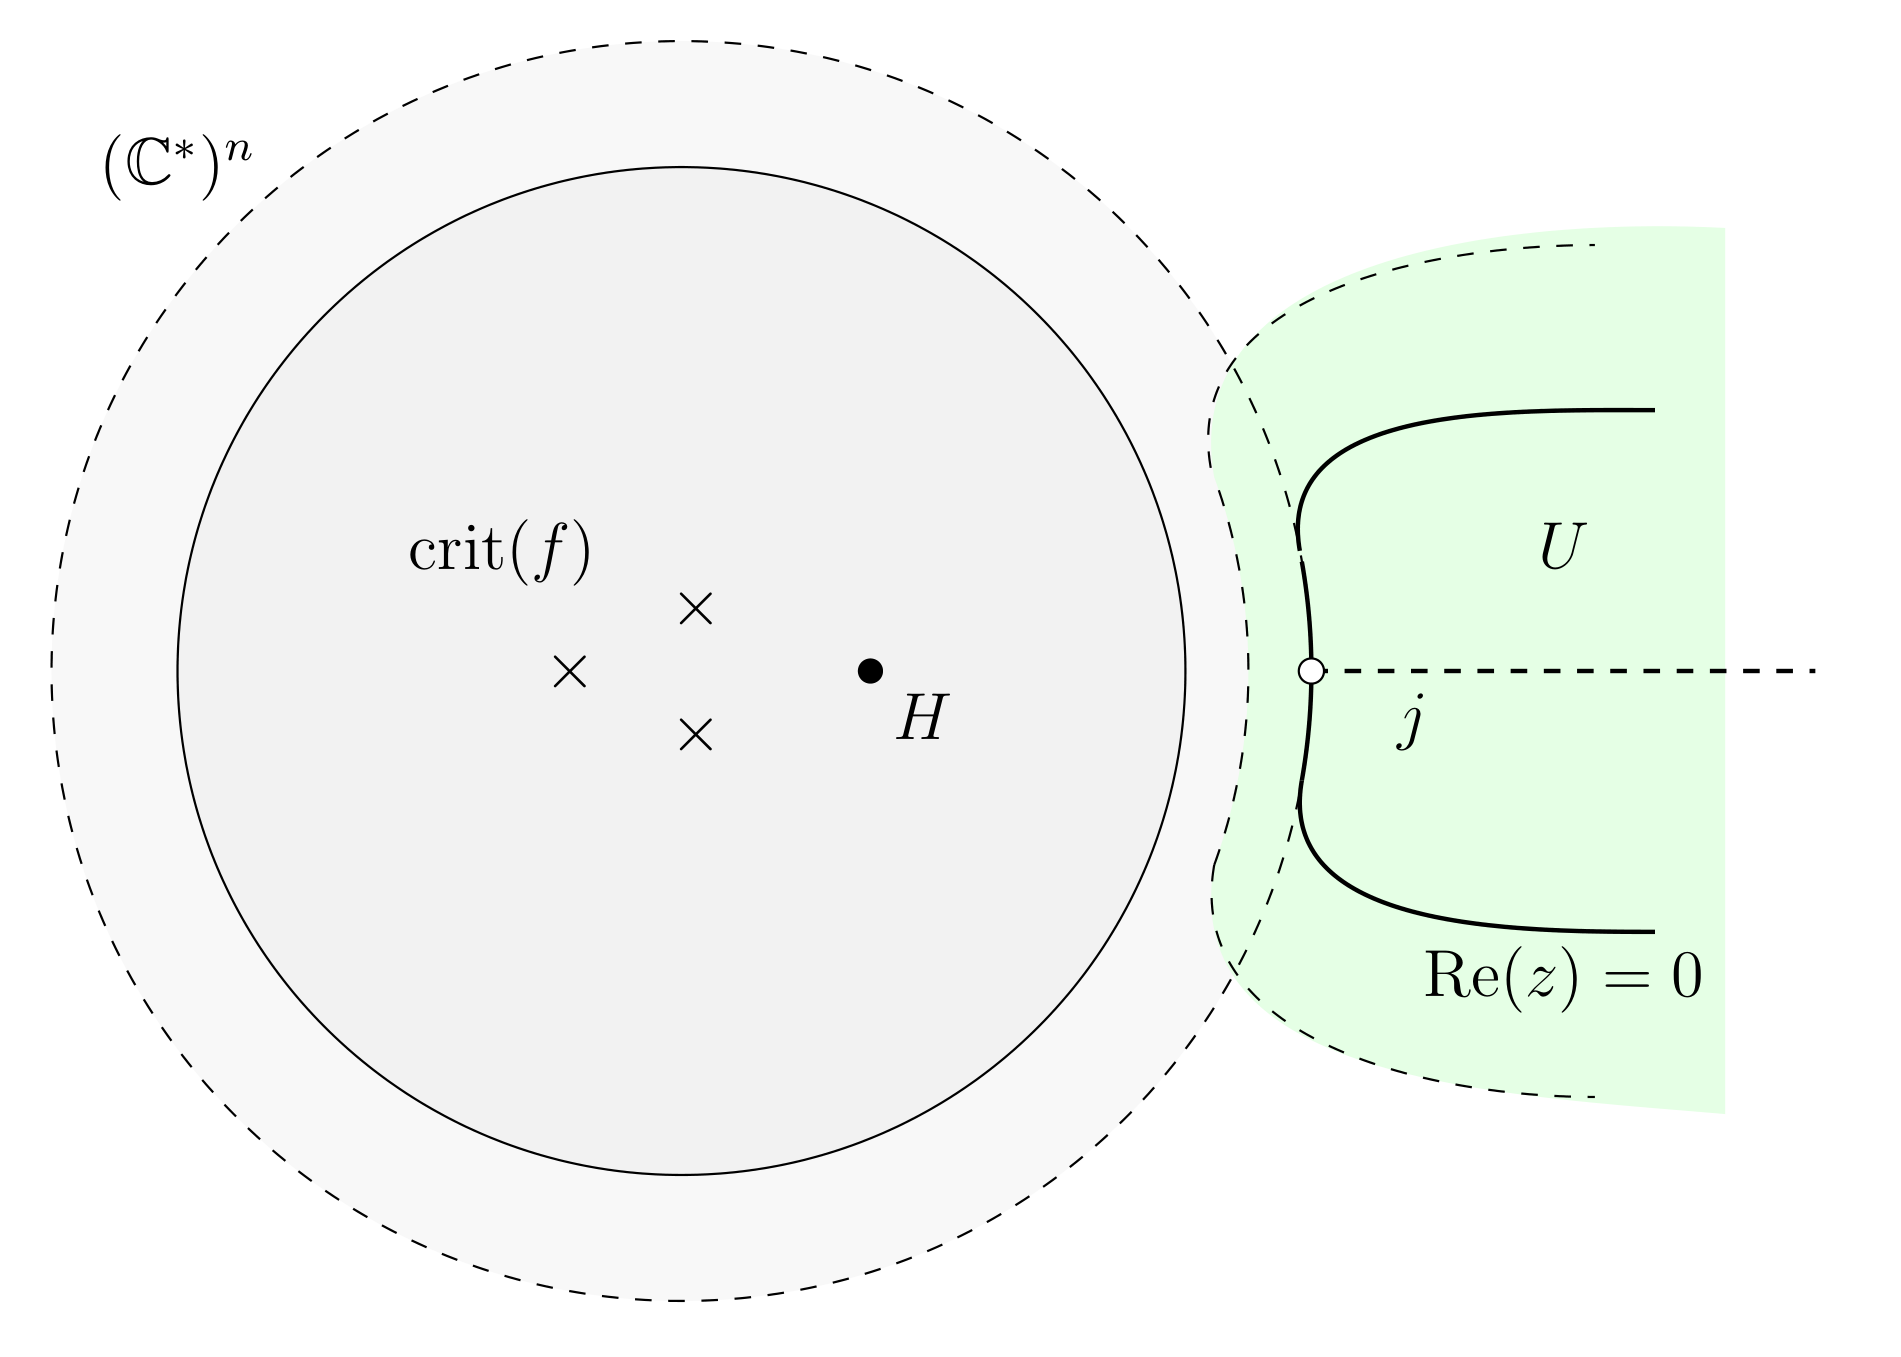
\includegraphics[width=0.52\textwidth]{figures/fig9_1.png}
\caption{提升函子 $j$ 对应于沿虚线水平线搬运拉格朗日对象：该虚线从穿孔出发，沿正实轴
延伸到 $\infty$。}
\label{fig:9-1}
\end{figure}

\begin{remarkx}
也可以定义负提升函子（negative lifting functor）
\[
j_-\colon\cW(H)\longrightarrow\cW(H\times A_1)\longrightarrow\cW((\C^*)^n\setminus H),
\]
其构造是：先与 $\R_{\le0}$ 作乘积并柱化，再作扇形包含（见图 \ref{fig:9-2}）。这一负提升
函子 $j_-$ 与提升函子 $j$ 相差一个扭转，即由 $f$ 绕 $\infty$ 的逆时针单值性 $\mu$ 给出的
扭转。
\end{remarkx}

\transnote{易错预警：原文在 $j_-$ 的中间范畴里写的是 $H\times A_1$，而在 $j$ 的定义里写的是
$H\times\C^*$；$A_1$ 在本节未另作说明，宜照原文录下，不要擅自改写成 $\R_{\le0}$——后者只
出现在紧随其后的柱化步骤中。}

\begin{theorem}\label{thm:9-0-2}
提升函子 $j\colon\cW(H)\to\cW_0((\C^*)^n\setminus H)$ 镜像于
\[
j_{D*}p_D^*\colon\operatorname{Coh}(D)\longrightarrow\operatorname{Coh}(Z),
\]
其中镜像等价取定理 \ref{thm:8-2-1} 中的 $\cW_0((\C^*)^n\setminus H)\to\operatorname{Coh}(Z)$；
这里 $j_D\colon K_X|_D\to Z$ 与 $p_D\colon K_X|_D\to D$ 分别是包含映射与投影。
\end{theorem}

% ===== 原书 p.130 =====

\begin{figure}[htbp]
\centering
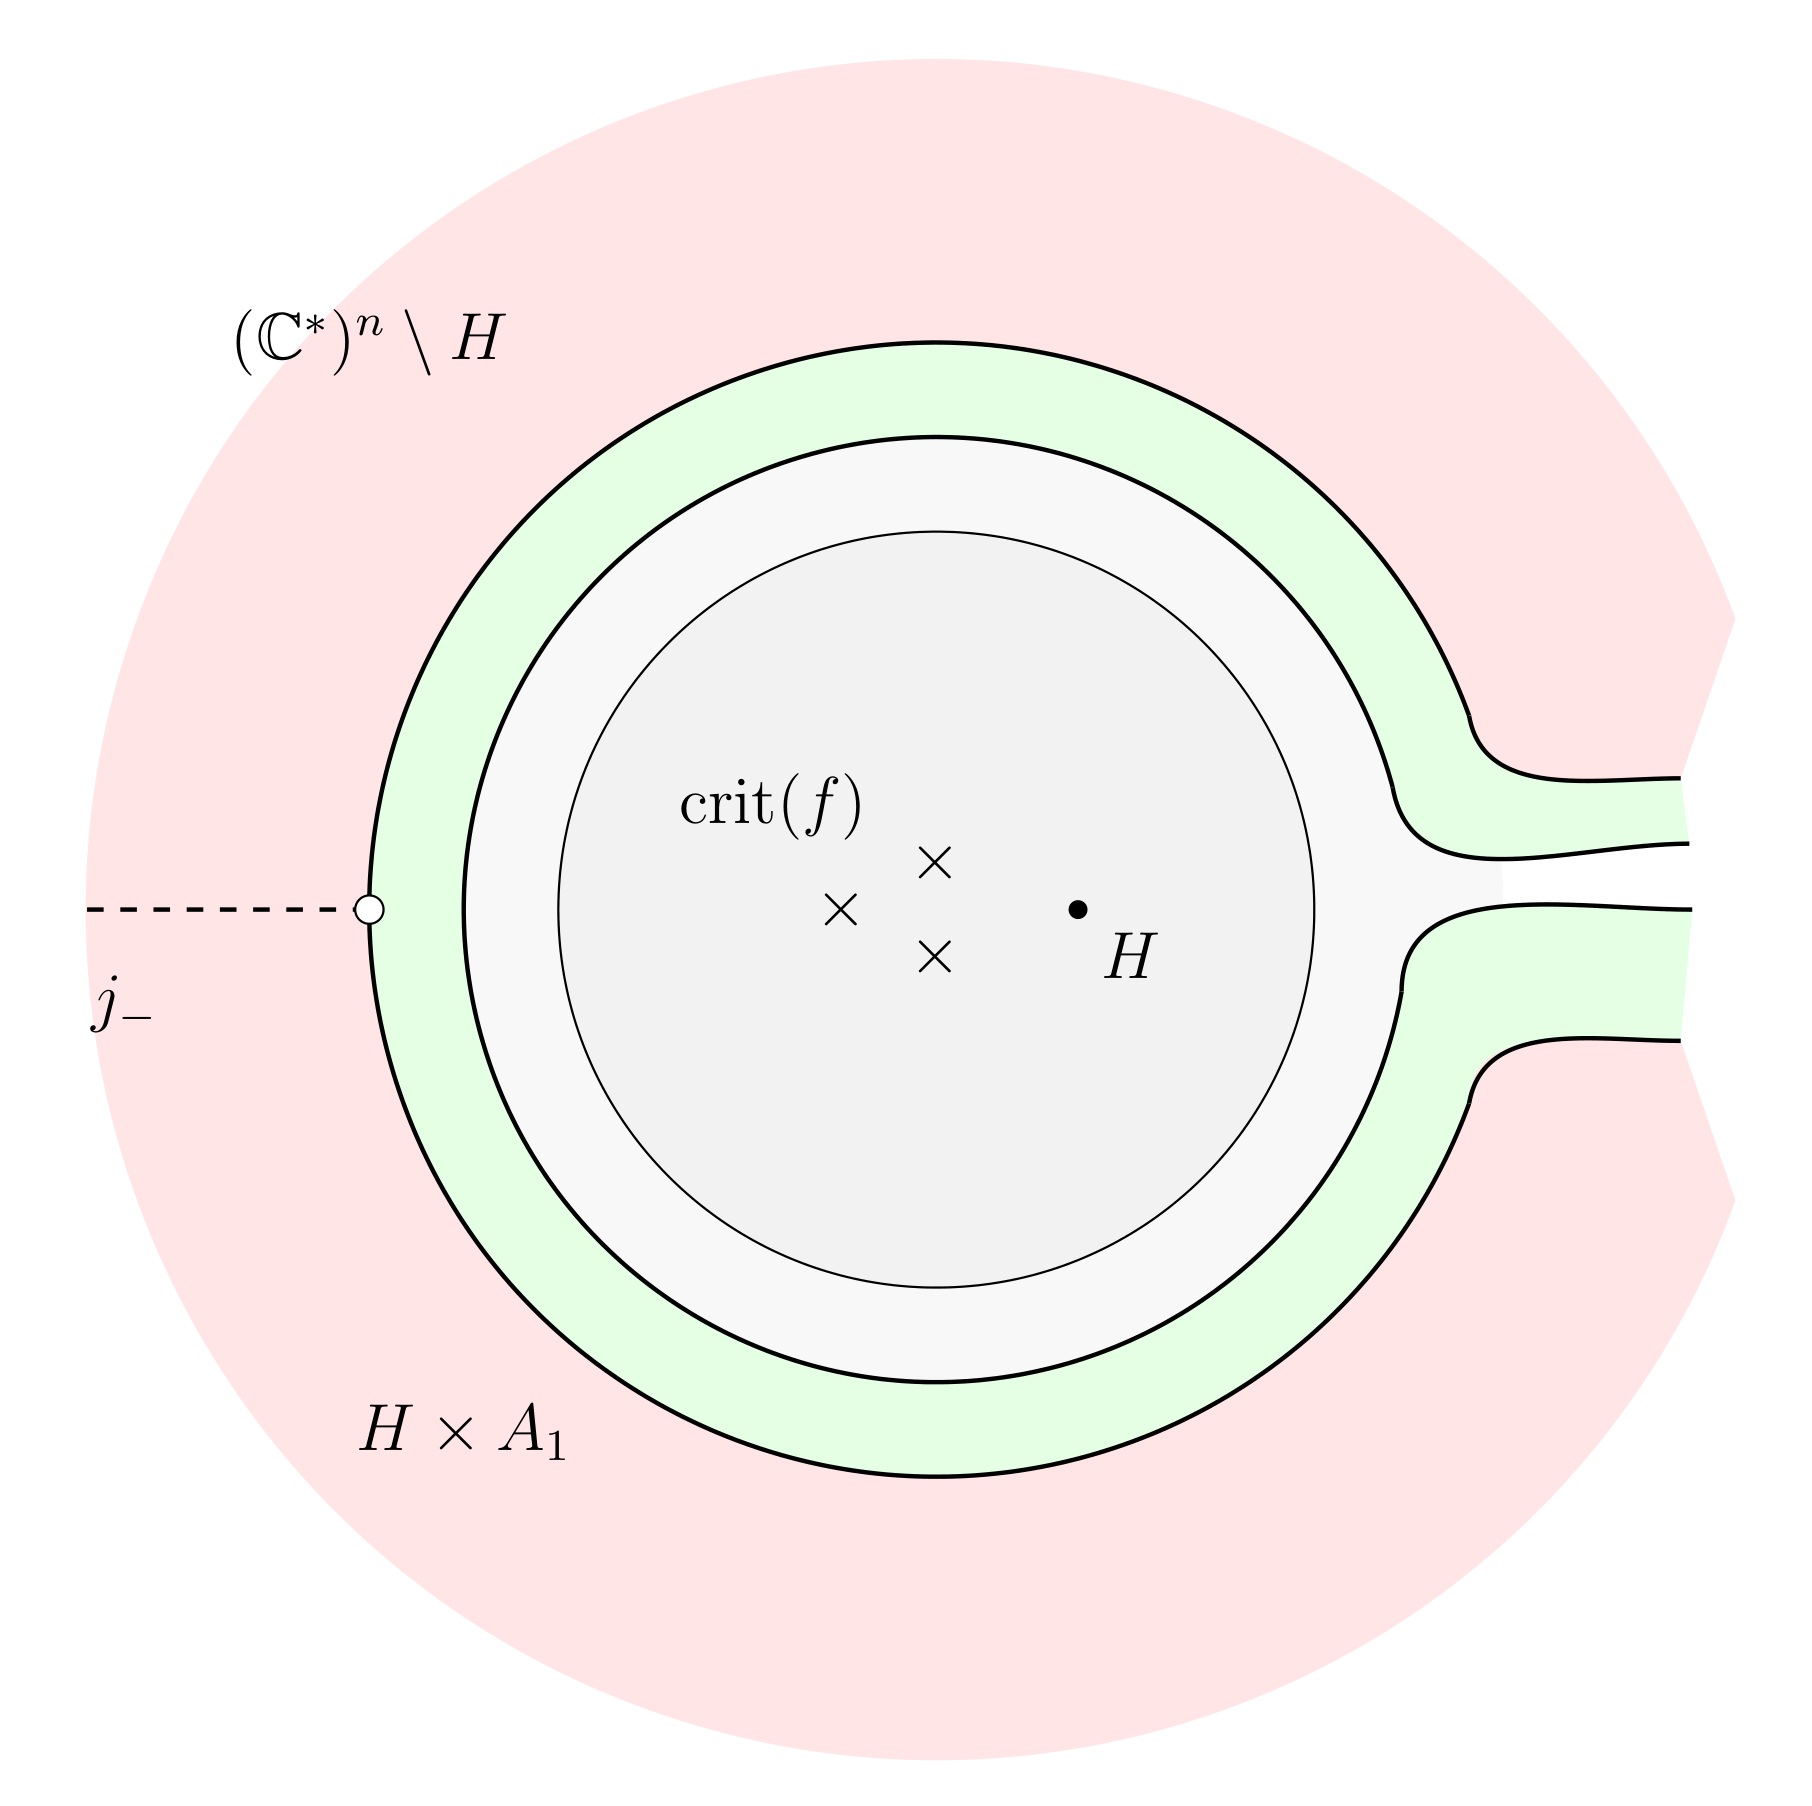
\includegraphics[width=0.42\textwidth]{figures/fig9_2.png}
\caption{负提升函子 $j_-$ 对应于沿虚线水平线搬运拉格朗日对象：该虚线从穿孔出发，延伸到
$-\infty$。}
\label{fig:9-2}
\end{figure}

% ===== 原书 p.131 =====

\begin{proof}
先考虑下面的图：
\[
\begin{tikzcd}[row sep=2.4em, column sep=1.5em]
\cW(H) \arrow[r,"\times\R_{\le0}"] \arrow[d,"\sim"] & \cW(H\times\C^*(2),z)
\arrow[r] \arrow[d,"\sim"] & \cW_0((\C^*)^n\setminus H) \arrow[d,"\sim"] \\
\operatorname{Coh}(D) \arrow[r,"p_{\tilde D}^*"] & \operatorname{Coh}(D\times\mathbb A^1[-1])
\arrow[r,"j_{\tilde D*}"] & \operatorname{Coh}(\tilde Z)
\end{tikzcd}
\]
右边的方块由定理 \ref{thm:7-2-4} 中的图而交换。左边的方块也交换，因为两个函子都对应于与
$\C[z]$（$|z|=2$）作张量。于是 $j\colon\cW(H)\to\cW_0((\C^*)^n\setminus H)$ 镜像于
$j_{\tilde D*}p_{\tilde D}^*\colon\operatorname{Coh}(D)\to\operatorname{Coh}(\tilde Z)$。
接下来由引理 \ref{lem:8-1-1}：在 Knörrer 等价 $\operatorname{Coh}(\tilde Z)\to
\operatorname{Coh}(Z)$ 之下，$j_{\tilde D*}p_{\tilde D}^*$ 再次被送到 $j_{D*}p_D^*$。
\end{proof}

\transnote{易错预警：交换图里带波浪号的箭头是范畴等价，不是同构的自然变换；同时注意
$\tilde D$ 与 $D$、$\tilde Z$ 与 $Z$ 的区别——定理的结论里落到的是不带波浪号的
$j_{D*}p_D^*$，带波浪号的那个只是证明中途的对象。}

\transnote{背景直觉：交换图里 $\C^*(2)$ 括号中的 2 表示该 $\C^*$ 因子的分次权重为 2，即其坐标 $z$ 满足 $|z|=2$；下文「与 $\C[z]$（$|z|=2$）作张量」正是对这一记号的说明。}

\begin{remarkx}
由于单值性带来的扭转，在 $\cW_0((\C^*)^n\setminus H)$ 与 $\operatorname{Coh}(Z)$ 的
镜像等价之下，负提升函子 $j_-$ 会镜像于 $j_{D*}p_D^*(K_X^{-1}|_D\otimes\cdot)$。理由如下：
由命题 \ref{prop:7-2-1}，逆时针单值性 $\mu$ 镜像于与 $K_X^{-1}|_D$ 作张量。这一结论对应于
猜想 \ref{conj:aur-funct} 的第 (4) 条。
\end{remarkx}

\transnote{易错预警：$K_X^{-1}|_D\otimes\cdot$ 表示先取 $K_X^{-1}$ 在 $D$ 上的限制，再与
对象作张量；它不是 $K_X^{-1}|_D$ 与某个固定对象的张量积，也不是 $K_X|_D$ 的逆。}

\begin{lemma}\label{lem:9-0-3}
存在 $\operatorname{Coh}(X)\to\operatorname{Coh}(Z)$ 的函子正合三角形：
\[
\begin{tikzcd}[row sep=1.0em, column sep=3.4em]
{j_{D*}p_D^*i_D^*} \arrow[rr,"+1"] & & i_{X*} \arrow[dl] \\
& \pi_X^* \arrow[ul] &
\end{tikzcd}
\]
\end{lemma}

\begin{proof}
映射 $i_{X*}\cF\to\pi_X^*\cF$ 是子层包含（subsheaf inclusion）：其余核恰是限制 $\cF|_D$ 沿投影
$K_X|_D\to D$ 的拉回。
\end{proof}

\transnote{含糊点拨：原文只画出三角形而未写循环方向。按本页的箭头读，它是
$\pi_X^*\to j_{D*}p_D^*i_D^*\xrightarrow{+1}i_{X*}\to\pi_X^*$；$+1$ 标在从第三个顶点
出发的那条箭头上，表示该映射带分次移位 1。}

\begin{corollary}\label{cor:9-0-4}
存在正合三角形，把作为函子 $\cW((\C^*)^n,f)\to\cW_\infty((\C^*)^n\setminus H)$ 的
$\alpha_0$、$\alpha_\infty$ 与 $j\cap$ 联系起来：

% ===== 原书 p.132 =====

\[
\begin{tikzcd}[row sep=1.0em, column sep=3.4em]
{j\cap} \arrow[rr,"+1"] & & \alpha_0 \arrow[dl] \\
& \alpha_\infty \arrow[ul] &
\end{tikzcd}
\]
并且对 $\cW_0((\C^*)^n\setminus H)$ 与 $j_-$ 有相应的正合三角形。
\end{corollary}

\transnote{易错预警：本三角形的三个顶点排布是 $j\cap$、$\alpha_0$（右上）、$\alpha_\infty$
（下方）。按箭头读，循环为 $\alpha_\infty\to j\cap\xrightarrow{+1}\alpha_0\to\alpha_\infty$。
不要与 §1.6 中同型三角形的排布混看，那里 $\alpha_0$ 与 $\alpha_\infty$ 的位置相反。}

\begin{proof}
这正是引理 \ref{lem:9-0-3} 的镜像：用定理 \ref{thm:8-2-1} 可知 $\pi_X^*$ 镜像于
$\alpha_\infty$。
\end{proof}

\subsection{一个例子}

本节的例子取 $H=\{-1\}$，篇幅虽短，却足以显示 $[1]$-移位与不同 $\Z$-分次为何必要。
先在 B 侧作如下等同：
\begin{itemize}[leftmargin=2em,itemsep=0.2em]
\item $X=\operatorname{Spec}(\C[x])$；
\item $K_X=\operatorname{Spec}(\C[x,y])$；
\item $\mathbb A^1[-1]=\operatorname{Spec}(\C[t])$，$|t|=-1$。
\end{itemize}

在 A 侧，$\Pi_1=\C^*\setminus H$ 有两种不同的粘合展示，分别由命题 \ref{prop:7-1-1} 与
命题 \ref{prop:7-1-2} 给出，如图 \ref{fig:9-3} 所示。此时两种分次的选择容易描述：
\[
\eta_0=\frac{\dd z}{z},\qquad\qquad \eta_\infty=\frac{\dd z}{z(z+1)}.
\]
对 $\eta_0$ 而言，绕 $-1$ 的简单顺时针 Reeb 轨道次数为 2，绕另外两个穿孔的相应轨道次数
为 0。

% ===== 原书 p.133 =====

\begin{figure}[htbp]
\centering
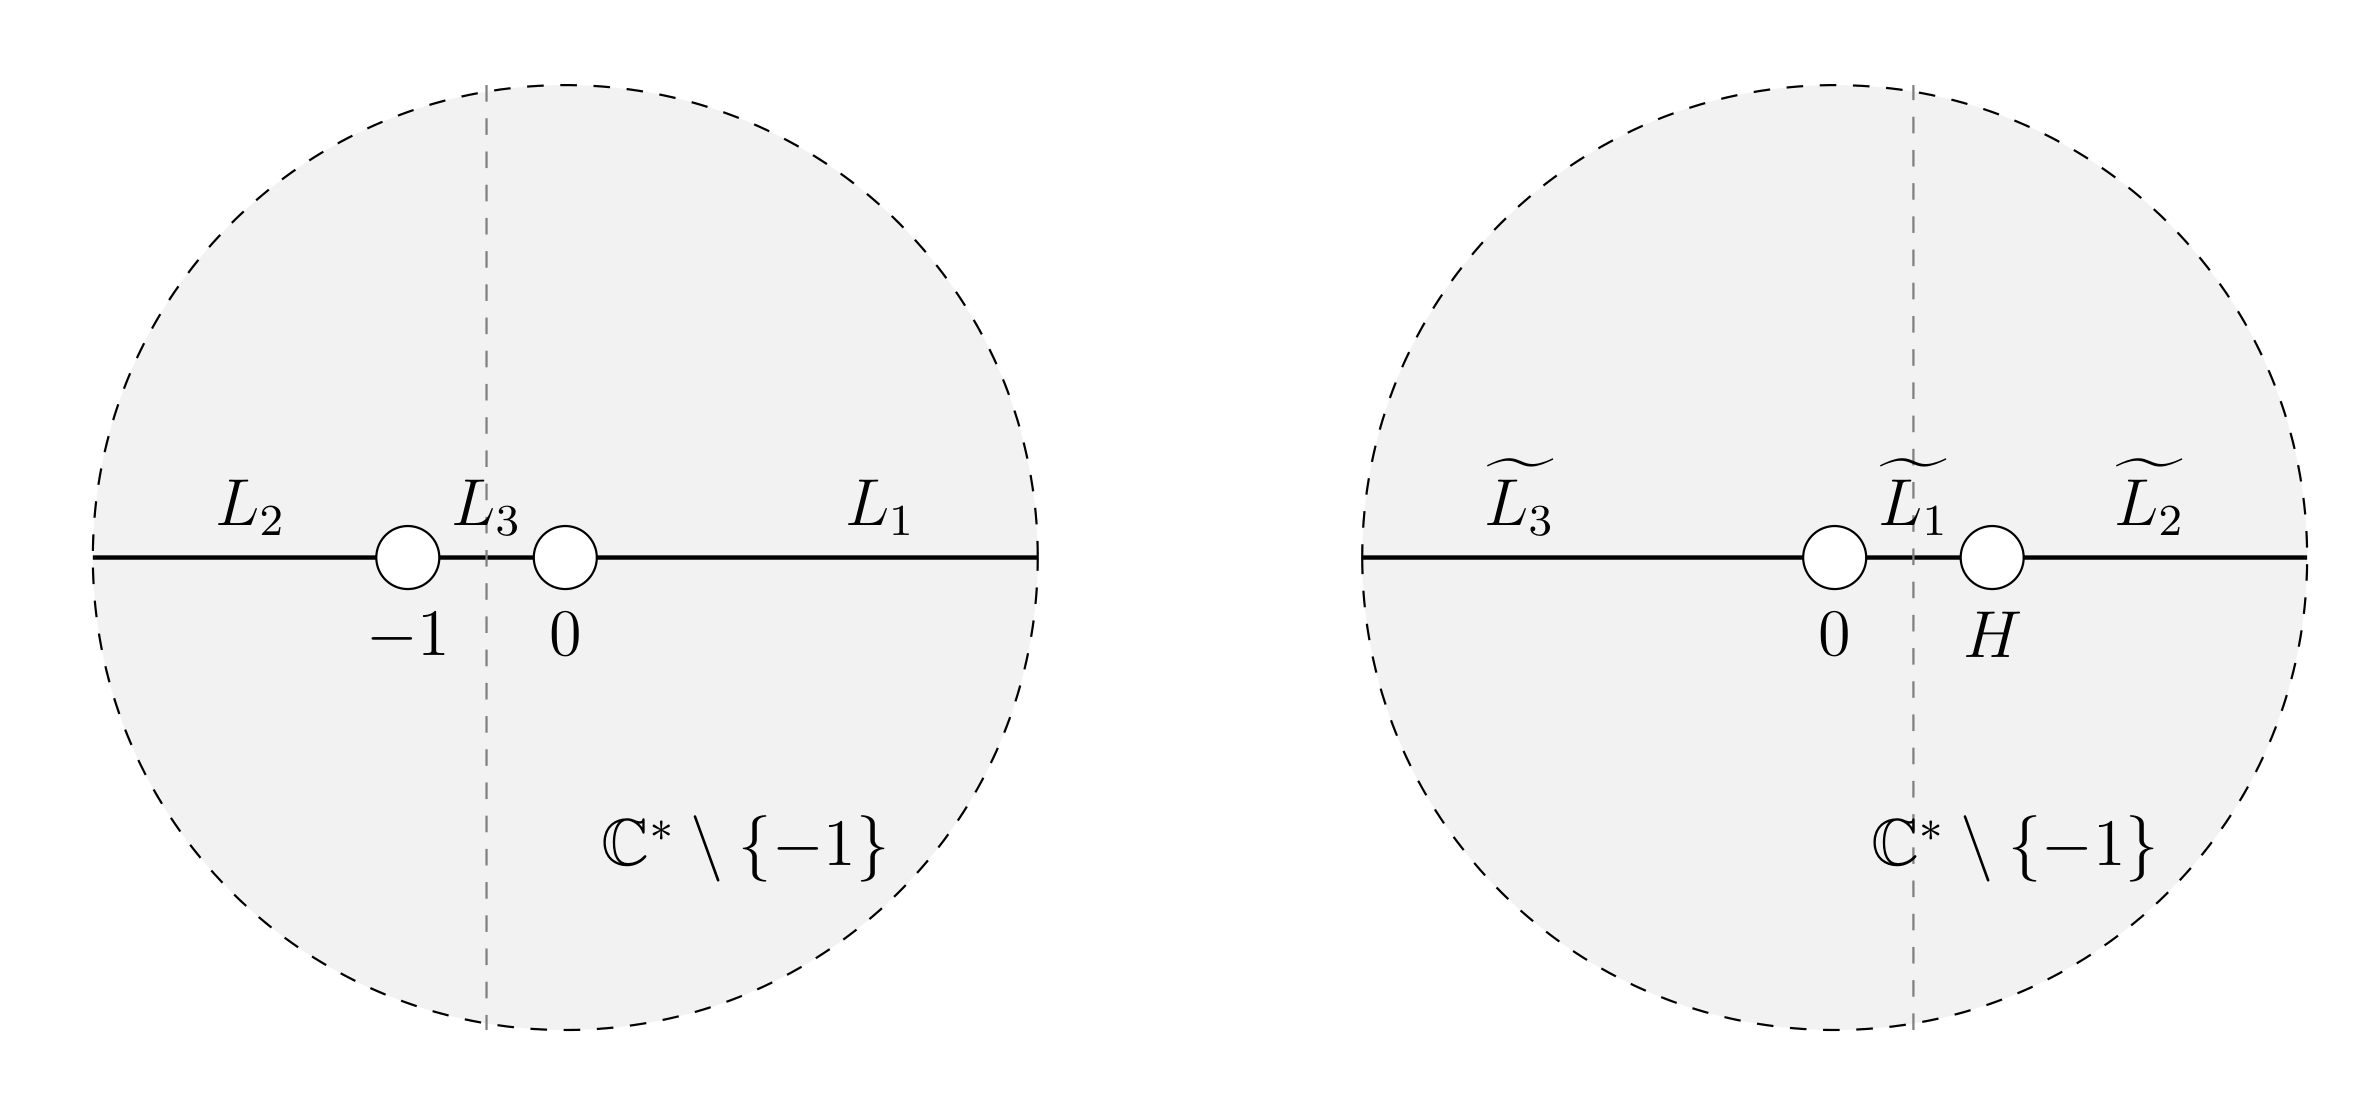
\includegraphics[width=0.78\textwidth]{figures/fig9_3.png}
\caption{裤子（pair of pants）的两种粘合展示，分别来自 $\tilde f_0$ 与 $\tilde f_\infty$
（从左到右），图中标出生成拉格朗日对象。虚线竖线表示划分两个子扇形的扇形超曲面。}
\label{fig:9-3}
\end{figure}

对 $\eta_\infty$ 则情形相反：绕 $\infty$ 的简单顺时针 Reeb 轨道次数为 2。希望这能部分
解释我们所选取的记号。这也提示：在不太正式的意义上，等价
$\cW_0(\Pi_1)\to\cW_\infty(\Pi_1)$ 会「交换零与无穷」。

\transnote{易错预警：$\eta_0$ 与 $\eta_\infty$ 是同一个补集上两个不同的平凡化，因而给出
两个\emph{不同的} dg 范畴 $\cW_0(\Pi_1)$ 与 $\cW_\infty(\Pi_1)$；下标 0、$\infty$ 指的是
分次所用平凡化，不是某种极限。}

如图 \ref{fig:9-3} 所示，我们用 $L_1,L_2,L_3$ 记取 0-分次的 wrapped Fukaya 范畴的一组
生成拉格朗日对象（generating Lagrangians），用 $\tilde L_1,\tilde L_2,\tilde L_3$ 记取 $\infty$-分次的相应对象。
事实上可以证明：与 Knörrer 周期性等价 $\operatorname{Coh}(Z)\to\operatorname{Coh}(\tilde Z)$
复合，会把 $L_i$ 与 $\tilde L_i$ 互换。特别地，$j_-$ 将对应于 $j$；一般情形下，这会涉及
单值性的扭转。

\transnote{含糊点拨：“$j_-$ 将对应于 $j$”是一句简写：两者的镜像只在复合 Knörrer 等价并
作单值性扭转之后才一致。原文紧接的“一般情形下”正是指这个扭转，读时不要理解成 $j_-=j$。}

\begin{proposition}\label{prop:9-1-1}
在定理 \ref{thm:7-2-4} 与定理 \ref{thm:8-2-1} 所诱导的镜像对称等价之下，有
\begin{itemize}[leftmargin=2em,itemsep=0.2em]
\item $\alpha_\infty(L_1)\mapsto\pi_{\mathbb A^1_x}^*(\cO_{\mathbb A^1_x})[1]$，

% ===== 原书 p.134 =====

\item $\alpha_0(\tilde L_2)\mapsto i_{\mathbb A^1_x*}(\cO_{\mathbb A^1_x})$，
\item $\rho(L_2)\mapsto q(\cO_{\mathbb A^1_y})$；
\item $j(\C)\mapsto\pi_{\mathbb A^1_y}^*(\cO_0)$。
\end{itemize}
\end{proposition}

\transnote{易错预警：这一组公式里 $\mathbb A^1_x$ 与 $\mathbb A^1_y$ 的下标并不统一——前
两条用 $x$，后两条用 $y$。这是原文的写法，照录；不要把它们“统一”成同一个坐标。}

\begin{proof}
按定义，$\alpha_\infty$ 把 $\cW(\C^*,z)$ 的唯一生成元 $L_1$ 送到 $\cW_0(\Pi_1)$ 中的
$L_1$；同样，$\alpha_0$ 把 $\cW(\C^*,z)$ 的生成元送到 $\cW_\infty(\Pi_1)$ 中的
$\tilde L_2$。在粘合诱导的镜像等价之下，前者被送到模 $\C[x]$ 到
$\mathbb A^1\cup_0\mathbb A^1[-1]=\tilde Z$ 的推出。同样，$\tilde L_2$ 作为
$\C[x,y]/(xy)$-模对应于 $\C[x]$，这就验证了 $\alpha_0$ 与 $i_{X*}$ 的对应。

接下来需要理解 Knörrer 周期性等价
\[
\operatorname{Coh}\C[x,y]/(xy)\longrightarrow
\operatorname{Coh}_{\mathbb G_m}(\mathbb A^1\times\mathbb A^1\times\mathbb A^1,xyt)
\longleftarrow\operatorname{Coh}\C[x,t]/(xt).
\]
在这一等价下，$\operatorname{Coh}(\mathbb A^1\cup_0\mathbb A^1[-1])$ 中的 $\C[x]$ 被送到
下面的矩阵分解：
\[
\begin{tikzcd}[row sep=1.4em, column sep=5em]
\C[x,y,t] \arrow[rr,bend left=20,"t"] & & \C[x,y,t] \arrow[ll,bend left=20,"xy"']
\end{tikzcd}
\]
它是下列矩阵分解的 $[1]$-移位：
\[
\begin{tikzcd}[row sep=1.4em, column sep=5em]
\C[x,y,t] \arrow[rr,bend left=20,"xy"] & & \C[x,y,t] \arrow[ll,bend left=20,"t"']
\end{tikzcd}
\]
而后者又是 $\operatorname{Coh}(\mathbb A^1\cup_0\mathbb A^1)$ 中 $\C[x,y]/(xy)$ 的像
（注意 $t$ 的权为 1 这一点要紧）。这一模沿投影 $\mathbb A^1\cup_0\mathbb A^1\to\mathbb A^1$
从 $\operatorname{Coh}(X)$ 的生成元 $\C[x]$ 拉回。
\end{proof}

\transnote{含糊点拨：两幅来回箭头的图是矩阵分解的简写——一对模配上两条映射。前一幅的
上方箭头为 $t$、下方箭头为 $xy$，后一幅把二者对调；对调恰是 $[1]$-移位的效果，因此文中
说前者是后者的 $[1]$-移位。}
